\documentclass[titlepage,10pt,a4paper]{article}
\usepackage[utf8]{inputenc}
\usepackage{graphicx}
\usepackage{hyperref}
\usepackage[ngerman]{babel}
\usepackage{float}
\usepackage{subcaption}
\usepackage{listings}
\usepackage{color}

\usepackage{glossaries}
\makeglossaries


\title{Validierungsbericht}
\date{\today{}, Passau}

\begin{document}
\begin{titlepage}
\vspace*{3cm}
\begin{center}
\textbf{\textsc{\LARGE Validierungsbericht}}

{\large \today}

\vspace{2cm}
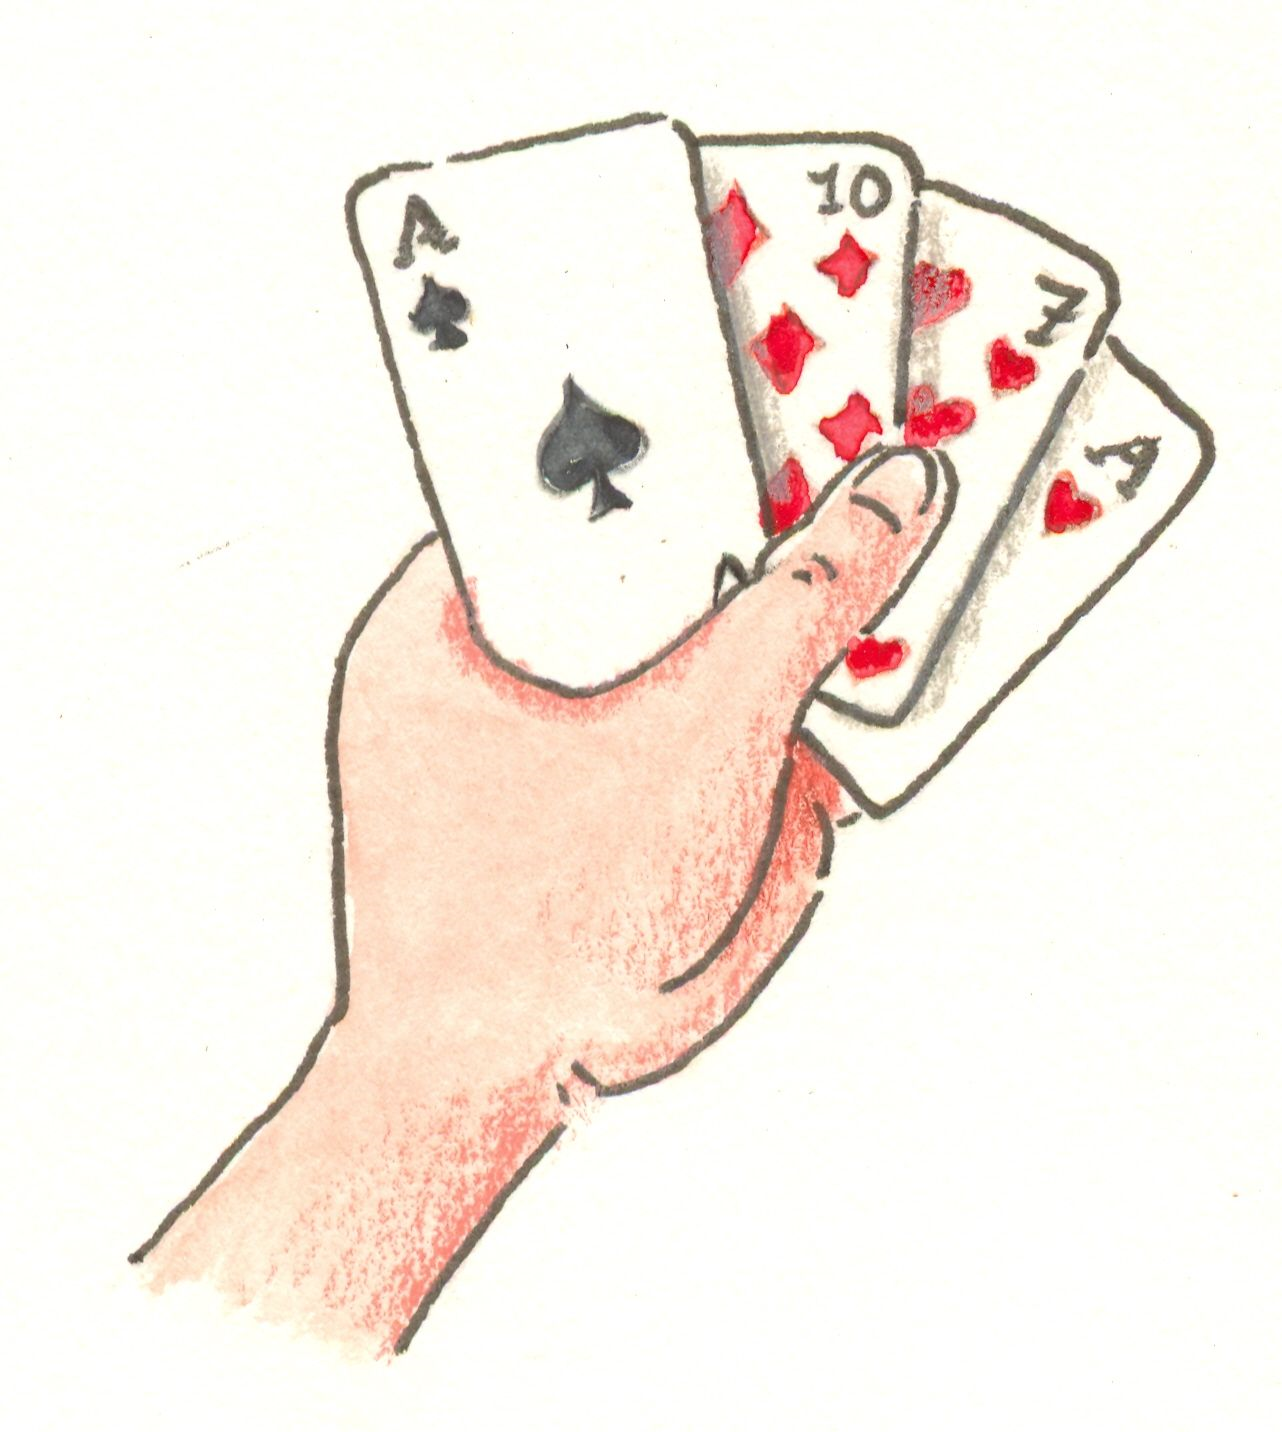
\includegraphics{kartenspiel}
\ \\
\ \\

\textbf{\textsc{\LARGE NET-WizHearts}}
\vspace{2cm}

\begin{tabular}{|c|c|c|}\hline
   Phase & Verantwortlicher & E-Mail \\ \hline\hline
   Pflichtenheft & Alina Meixl &  alina@meixl.de \\ \hline
   Entwurf & Viktoria Witka & witkaviktoria@freenet.de \\ \hline
   Spezifikation & Daniel Riedl & dariedl14@yahoo.de \\ \hline
   Implementation & Andreas Altenbuchner& a.andi007@gmail.com\\ \hline
   Validierung & Patrick Kubin & kubin@fim.uni-passau.de\\ \hline
   Präsentation & w& w\\ \hline
 \end{tabular}
\vspace{2cm}
\\
\end{center}
\end{titlepage}
\tableofcontents
\pagenumbering{arabic}
\hypersetup{pageanchor=true}

\newpage
 
\section{Einleitung}
Im folgenden Dokument werden alle Tests und ihre Ergebnisse aufgeführt, die im Rahmen der Testphase des Spiels NET-WizHearts getätigt wurden um die Funktionalitäten des Programms testen und deren Korrektheit zu bestätigen.
\section{Plichtenheft Tests}
	\subsection{Wizard}
	\subsection{Hearts}
\section{Line- und Branch-Coverage}
	\subsection{Line-Coverage}
	\subsection{Branch-Coverage}
\section{Korrektheitstests}
\section{Skalierungs- und Belastungs-Tests}
\section{Weitere Tests}
	\subsection{Test durch freie zusätzliche Testgruppen}

\newpage
\printglossaries

\end{document}